% Header
%HEADER
\def\makroEinseitig{
	%KOMA-Script-Klasse: scrreprt
	%deutsches Design, Schriftgröße 12, DIN A4
	%Literaturverzeichnis und Index in Inhaltsverzerzeichnis einbinden
	\documentclass[12pt,a4paper,listof=totoc,oneside]{scrreprt}

	%Seitenspiegel einstellen
	\usepackage[a4paper]{geometry}
	\geometry{a4paper,left=30mm,right=25mm,bottom=20mm,top=15mm,bindingoffset=2mm,includehead,includefoot}
}

\def\makroFH-Kopfzeilenstil{
	\pagestyle{scrheadings}
	\setheadsepline{0.4pt}
	\pagestyle{scrheadings}
	\renewcommand*{\chapterpagestyle}{scrheadings}
}

\makroEinseitig{}

% passende Codierung
\usepackage[utf8]{inputenc}

% schalte Umlaute frei
\usepackage[ngerman]{babel}

% wird gebraucht für richtige Umlaute 1)
\usepackage{pslatex}

% wird gebraucht für richtige Umlaute 1)
\usepackage[T1]{fontenc}

% Mathematik
\usepackage{amsmath}

% Symbole
\usepackage{amssymb}

% Griechische Symbole
\usepackage{upgreek}

% weitere Symbole
\usepackage{pxfonts}

% Phonetischen Alphabete für LaTeX
\usepackage{tipa}

% farbige Schriften
\usepackage{color}

% scrhack redefines macros of packages from other authors!
\usepackage{scrhack}

% Bilder fixieren
\usepackage{float}

% Grafiken einbinden
\usepackage{graphicx}

% Kopf- und Fußzeilen
\usepackage[automark,standardstyle,markusedcase]{scrpage2}

% deutsche Überschriften
\usepackage[ngerman]{translator}

% deutsche Anführungszeichen
\usepackage[autostyle=true,german=quotes]{csquotes}

% Kopfzeilenabstand festlegen
\setlength{\headheight}{10mm}

% Captions
\usepackage{caption3}
\usepackage{caption}

% Für Deutsch Abb. & Tab.
\addto\captionsngerman{
	\renewcommand{\figurename}{Abb.}
	\renewcommand{\tablename}{Tab.}
}

% Glossar-Package (keine Seitenzahlen, Abkürzungsverzeichnis, ins Inhaltsverzeichnis)
\usepackage[nonumberlist,acronym,toc]{glossaries}

% Zitieren
\usepackage[numbers,square,sort]{natbib}

% Glossar einschalten
\makeglossaries{}

% für URLs
\usepackage{url}

% Links sollen nicht farbig sein
\usepackage[colorlinks=false]{hyperref}

% Code Beispiele
\usepackage{listings}

% Symbole
\usepackage{amssymb}

% Style für Listings
\lstset{frame=single,
captionpos=t,
numbers=left,
breaklines=true,
prebreak=\raisebox{0ex}[0ex][0ex]{\ensuremath{\hookleftarrow}},
numberstyle=\tiny,
basicstyle=\fontfamily{pcr}\selectfont\footnotesize}

% Um besser Tabellen zu gestalten
\usepackage{colortbl}
\definecolor{light-gray}{gray}{.8}
\definecolor{lighter-gray}{gray}{.9}
\definecolor{lightgreen}{rgb}{0.56, 0.93, 0.56}

\usepackage{booktabs}
\usepackage{tabularx}

\newcommand{\Storycard}[6]{
	\begin{table}[H]
		\framebox{
			\begin{tabularx}{\textwidth}{l|l|l}
			\textbf{Nr:} #1 & \textbf{Story Points:} #2 Pkt. & \textbf{Priorität:} #3 \\
			\hline
			\multicolumn{3}{p{0.97\textwidth}}{\textbf{Titel:} #4} \\
			\hline
			\multicolumn{3}{p{0.97\textwidth}}{\textbf{Beschreibung:} #5} \\
			\hline
			\multicolumn{3}{p{0.97\textwidth}}{\textbf{Akzeptanztests:} #6} \\
			\end{tabularx}
		}
	\end{table}
}

% Dokument interne Referenzen
\newcommand*{\fullref}[1]{\hyperref[{#1}]{\autoref*{#1} \nameref*{#1}}}

% Fügt bei Zahlen kleiner 10  eine 0 vorne dran
\newcommand{\leadingzero}[1]{\ifnum #1<10 0\the#1\else\the#1\fi}

% ISO Datum im Format YYYY-MM-DD
\newcommand{\todayiso}{\the\year–\leadingzero{\month}–\leadingzero{\day}}

% Kein Einrücken beim Beginn eines Paragraphen (z.B. nach einem Bild)
\setlength{\parindent}{0pt}

% Inkludiere Einstellungen
\newcommand{\thesis}{Masterarbeit}
\newcommand{\name}{Vetter}
\newcommand{\vorname}{Alexander}

\newcommand{\batitle}{Reactive Design Patterns}
\newcommand{\babetreuer}{Prof.\ Dr.\ Gudrun Schiedermeier}



% Kopfzeilenstil
\makroFH-Kopfzeilenstil

% 1.5 Zeilenabstand
\renewcommand{\baselinestretch}{1.5}\normalsize

\begin{document}

% Glossar
%Akronyme

%\newacronym{MOM}{MOM}{Message-oriented Middlware\protect\glsadd{glos:MOM}}

% Glossareinträge

\newglossaryentry{webscale}{
name={Web Scale},
description={Bezeichnet Anwendungen die aufgrund ihrer Architektur mit mehreren Millionen Nutzer zurecht kommen. Das Internet ermöglicht es, global erreichbare Software Systeme bereitzustellen}
}

\newglossaryentry{locationtransparency}{
name={Location Transparency},
description={Ist ein System \enquote{Location Transparent} dürfen die Komponenten und deren Kommunikation nicht von einem physikalischen Host oder anderen \enquote{örtlichen} Gegebenheiten abhängig sein}
}

\newglossaryentry{denialofservice}{
name={Denial of Service Angriff},
description={Ein Denial of Service Angriff hat zum Ziel eine Anwendung beispielsweise durch eine überdurchschnittliche Anzahl von Anfragen mutwillig unnutzbar zu machen}
}

\newglossaryentry{messagequeue}{
name={Message Queue},
description={Eine Message Queue ist eine Datenstruktur bzw. ein Zwischenspeicher für Nachrichten in einer bestimmten Reihenfolge. Diese werden bis zu deren Abarbeitung in der Queue vorgehalten}
}

\newglossaryentry{flowcontrol}{
name={Flow Control},
description={Als Flow Control werden allgemein unterschiedlichste Verfahren bezeichnet, mit denen der \enquote{Fluss} von Daten innerhalb eines System gesteuert und beeinflusst werden kann}
}

\newglossaryentry{concurrency}{
name={Concurrency},
description={Concurrency oder zu Deutsch Nebenläufigkeit ist die Fähigkeit eines Systems mehrere Operationen gleichzeitig oder scheinbar gleichzeitig ausführen zu können. Dabei können diese Operationen auch im Zusammenhang stehen}
}

\newglossaryentry{pipelining}{
name={Pipelining},
description={Beim Pipelining zerlegt ein Prozessor ein Maschinenbefehl in Teilaufgaben, die dann zum Teil parallel durchgeführt werden können}
}

\newglossaryentry{multitasking}{
name={Multitasking},
description={Multitasking bezeichnet die Fähigkeit eines Betriebsystems, mehrere Prozess quasi-parallel auszuführen. Die Prozesses werden in in sehr kurzen Zeitabständen abwechselnd Rechnenleistung zugewiesen. Es entsteht der Eindruck als würden die Prozesse gleichzeitig ausgeführt}
}

\newglossaryentry{mutualexclusion}{
name={Mutal Exclusion},
description={Mutal Exclusion oder wechselseitger Auschluss beschreibt verschiedene Verfahren, mit denen sichergestellt wird, dass kritische Abschnitte in einem Programm gleichzeitig oder verschränkt durch nebenläufige Prozesse ausgeführt werden}
}

\newglossaryentry{memorycorruption}{
name={Memory Corruption},
description={Memory Corruption entsteht durch ungewollte Veränderung von Datenstrukturen aufgrund von Fehlern in einem Programm}
}

\newglossaryentry{deadlock}{
name={Deadlock},
description={Der Begriff Deadlock bezeichnet einen ungewollten Zustand, bei dem eine zyklische Wartesituation zwischen mehreren Prozessen oder Threads auftritt. Jeder involvierte Prozess oder Thread wartet auf die Zuweisung einer Ressource, die jedoch durch einen anderen Teilnehmer belegt ist}
}

\newglossaryentry{starvation}{
name={Starvation},
description={Starvation beschreibt ein Problem der Concurrency bei dem ein Prozess oder ein Thread benötigte Ressourcen nicht zugeweisen bekommt. Folglich kann dieser seine Arbeit nicht verrichten}
}

\newglossaryentry{contextswitching}{
name={Context Switching},
description={Context Switching beschreibt den Vorgang einen Betriebssystems bei dem ein Task, also ein Prozess oder ein Thread, unterbrochen wird und Rechenkapzität einem anderen Task zugeordnet wird. Dabei wird der Zustand und Ablauf des Tasks gesichert und durch den bereits gesicherten Context des anderen Tasks ersetzt}
}
\glsaddall{}

% Titelseite
%Titelseite

\thispagestyle{empty}

\begin{titlepage}

\vspace{3cm}

\begin{center}
	
\includegraphics[scale=0.8]{0-Template/Logo.pdf}
\end{center}

\vspace{2.5cm}

\begin{center}
	\large \textsc{Fakultät Informatik}
\end{center}

\vspace{1cm}

\begin{center}
	\huge \textbf{\thesis}
\end{center}

\vspace{1cm}

\begin{center}
	\large \textsc{\batitle}
\end{center}

\vspace{1cm}

\begin{center}
	\large \vorname{} \name{}
\end{center}

\vspace{4cm}

\begin{center}
	\large
	\textbf{Betreuerin: }\babetreuer%
\end{center}

\end{titlepage}


% Erklaerung
%Erklärung
\thispagestyle{empty}
\vspace{0.15cm}

\begin{center}
\textbf{\underline{ERKLÄRUNG ZUR \MakeUppercase{\thesis}}}
\end{center}

\vspace{0.25cm}

\begin{center}\large
\name, \vorname%
\end{center}

\vspace{0.25cm}

\begin{center}\huge
Hochschule Landshut\\
Fakultät Informatik
\end{center}

\vspace{0.1cm}

\begin{center}\large
Hiermit erkläre ich, dass ich die Arbeit selbständig verfasst, noch nicht anderweitig für Prüfungszwecke vorgelegt, keine anderen als die angegebenen Quellen oder Hilfsmittel benützt, sowie wörtliche und sinngemäße Zitate als solche gekennzeichnet habe.
\end{center}

\vspace{0.5cm}

\begin{center}
\begin{table}[h]
  \begin{tabular}{ll}
    {\todayiso}     & \ldots\ldots\ldots\ldots\ldots\ldots\ldots\ldots\ldots \\
    \textit{Datum}  & \textit{Unterschrift}
  \end{tabular}
\end{table}
\end{center}


% Abstract
% !TEX root = ../Masterdatei.tex
\begin{abstract}
\begin{center}
\Huge
\textit{\textbf{Abstract}}
\end{center}
\normalsize
\vspace{15mm}

Die vorliegende Arbeit beschäftigt sich mit Design Patterns, die die Eigenschaften des Reactive Manifestos erfüllen. Ziel der Arbeit wird es sein, Design Patterns zu identifizieren, die bei der Entwicklung von reaktiven Systemen von Nutzen sein können. Zu Beginn werden neu entstandene Anforderungen an Software Systeme erläutert, die die Motivation hinter dem Reactive Manifestos erklären. Für den Hauptteil werden die Grundlagen zu funktionaler Programmierung sowie den genauen Eigenschaften reaktiver Systeme dargelegt. Im Hauptteil werden dann eine Auswahl an Design Patterns genauer beleuchtet und festgestellt, ob diese die Eigenschaften des Reactive Manifestos erfüllen. Dazu werden dann Code Beispiele folgen, die den Umgang mit den Patterns in der jeweiligen Sprache darstellen sollen. Zum Schluss werden die Ergebnisse zusammen gefasst und ein Ausblick auf die Verwendung von reaktiven Systemen in moderner Softwarearchitektur gegeben.

\end{abstract}

% Thema und Zielsetzung
% Reaktive Design Pattern; Auswahl an Patterns und welche positive Eigenschaft haben sie, um die Entwicklung reaktiver Systeme zu unterstützen.

% Theorie
% Die Arbeit wird beantworten, ob und welche Eigenschaften des Reaktive Manifestos von einem Design Pattern erfüllt werden.

% Fragestellung
% Die Arbeit wird sich mit Reaktive Design Patterns beschäftigen, also ob und welche es gibt.

% Ergebnis & Fazit
% Fazit wird sein, dass es wichtig ist sich mit Reaktiven Systemen auseinander zu setzen, da sich die Anforderungen an Software bereits im Wandlen befinden. Concurrency und Parallelität gewinnen immer mehr an Bedeutung.
% !TEX root = ../Masterdatei.tex
\begin{abstract}
\begin{center}
\Huge
\emph{\textbf{Abstract}}
\end{center}
\normalsize
\vspace{15mm}

\textit{To be done.}

\end{abstract}


\clearpage
\begingroup
  \renewcommand*{\chapterpagestyle}{empty}
  \pagestyle{empty}
  \tableofcontents
  \clearpage
\endgroup

\setcounter{page}{1}

% Einleitung
% !TEX root = ../Masterarbeit.tex
\chapter{Einführung}\label{sec:einfuehrung}
Software wird entwickelt, um Probleme zu lösen und Aufgaben automatisiert zu erledigen --- ohne dabei menschliche Fehler zu machen. Deshalb ist es nicht verwunderlich, dass man an Software die Anforderung stellt, in angemessener Zeit auf Eingaben zu reagieren. Hierfür gibt es den Begriff \textit{responsiveness} (dt.\ Antwortbereitschaft)~\cite[S.~18]{kuhn_reactive_2015}.\\
Ein System, welches auf externe Ereignisse bzw. Eingaben antwortet (reagiert), nennt man reaktives System. David Harel und Amir Pnueli unterscheiden in ihrer Arbeit \enquote{On the Development of Reactive Systems} (1985) zwischen transformativen und reaktiven Systemen~\cite{harel_development_1985}. Transformative Systeme berechnen Ergebnisse einmalig auf der Basis bestimmer Eingabewerte (z.B. Compiler)~\cite[S.~2]{carkci_dataflow_2014}~\cite{wieringa_design_2003}. Reaktive Systeme definieren sie hingegen wie folgt:

\begin{quotation}
  Reactive systems [...] are repeatedly prompted by the outside world and their role is to continuously respond to external inputs~\cite{harel_development_1985}.
\end{quotation}

Folglich muss ein reaktives System, für die Dauer der Ausführung auf jede Eingabe bzw. Anfrage zeitnah reagieren. Üblicherweise handelt es sich bei reaktiven Systemen, um länger oder durchgehend laufende Applikationen. Hierzu zählen vor allem serverbasierte Anwendungen, die viele und häufig auch parallele Anfragen verarbeiten müssen.\\
In dieser Arbeit wird die Entwicklung von reaktiven Software Systeme behandelt, bei welchen die erwähnte \textit{responsiveness} und weitere Anforderungen von großer Bedeutung sind.

\pagebreak

\section{Wandel der Anforderungen}
Die heutigen Anforderungen an Software unterliegen dem rapiden Wachstum der Nutzung von Software im technischen, wie auch im sozialen Sinne. Der Wandel hin zu einer digitalen Gesellschaft und der weltweiten Vernetzung durch das Internet machen Software allgegenwärtig. Die Art und Weise, wie moderne Systeme implementiert werden, unterliegt ebenfalls diesem Wandel. Um den heutigen Ansprüchen zu genügen, müssen diese robuster, skalierbarer und anpassungsfähiger sein, als es früher der Fall war~\cite{boner_reactive_2014}.\\

Früher wurden mithilfe von Software überwiegend mathematische Probleme gelöst. Heutzutage sind die Aufgaben viel komplexer, nicht im Bezug auf mathematische Probleme, sondern vielmehr im Bezug auf die Menge der Daten~\cite[S.~18]{kuhn_reactive_2015}. Zum Beispiel muss der Kurznachrichten Dienst Twitter täglich über 500 Millionen Tweets\footnotemark[1] verarbeiten und über 300 Millionen Nutzern\footnotemark[2] auf der ganzen Welt zur Verfügung stellen. Netflix war im Dezember 2015 für rund 35~\%\footnotemark[3] des gesamten Internet-Traffics in Nordamerika verantwortlich. Das Internet ermöglicht es, global erreichbare Software Systeme bereitzustellen. Dies führt dazu, dass diese Systeme theoretisch mit ca. 3 Milliarden Nutzern\footnotemark[4] zurechtkommen müssen. Aufgrund der Zeitzonen existieren keine Wartungszeiträume, wie bei üblichen Software Installationen.

\footnotetext[1]{Twitter. Anzahl der täglichen Tweets auf Twitter vom Februar 2010 bis Oktober 2013 (in Millionen). http://de.statista.com/statistik/daten/studie/237226 (zugegriffen am 09. Januar 2016).}
\footnotetext[2]{Twitter. Anzahl der monatlich aktiven Nutzer von Twitter weltweit vom 1. Quartal 2010 bis zum 3. Quartal 2015 (in Millionen). http://de.statista.com/statistik/daten/studie/232401 (zugegriffen am 09. Januar 2016).}
\footnotetext[3]{Sandvine. Anwendungen mit dem größten Anteil am Internet-Datenverkehr in Nordamerika im Dezember 2015. http://de.statista.com/statistik/daten/studie/294315 (zugegriffen am 3. Juni 2016).}
\footnotetext[4]{Internet Live Stats. Anzahl der Internetnutzer weltweit von 1997 bis 2014 (in Millionen). http://de.statista.com/statistik/daten/studie/186370 (zugegriffen am 16. Februar 2016).}

\pagebreak

Die neuen Anforderungen, die durch das Internet und durch die rasant steigende Anzahl der Nutzer entstehen fast man unter dem Begriff \enquote{\gls{webscale}} zusammen. Die dafür nötigen Architekturansätze solcher skalierbarer Systeme halten auch Einzug in die Entwicklung von Enterprise Applikationen. Unternehmen benötigen mehr und mehr die technischen Konzepte, wie sie beispielsweise von Twitter und Netflix umgesetzt werden. Denn viele Unternehmen müssen mittlerweile mit immer größer werdenden Datenmengen zurechtkommen.\\

Neben der Skalierbarkeit unterliegen auch die Antwortzeiten dem Wandel der Anforderungen. Der Benutzer von heute ist es nicht mehr gewohnt, lange auf Ergebnisse warten zu müssen. Laut einer Umfrage unter Smartphone-Nutzern von 2011 würden 16~\% der Befragten eine aufgerufene Webseite wieder verlassen, wenn die Ladezeit mehr als drei Sekunden beträgt. Weitere 10~\% bei einer Ladezeit von mehr als vier Sekunden und nochmal weitere 28~\% bei mehr als fünf Sekunden\footnotemark[5]. Man kann davon ausgehen, dass Nutzer heute weitaus kürzere Ladezeiten erwarten und fordern.\\

\footnotetext[5]{Wie lange sind Sie bereit zu warten bis eine mobile Website auf Ihrem Smartphone vollständig geladen hat?. http://de.statista.com/statistik/daten/studie/202650 (zugegriffen am 09. Januar 2016).}

Ein weiterer Umbruch ist bei der Entwicklung von Prozessoren zu beobachten. Die Prozessorhersteller sind bei den Frequenzen bzw. Taktraten an Grenzen gestoßen, weshalb man seit einigen Jahren auf Multicore-Architekturen setzt. Für Software Entwickler bedeutet das, um Anwendungen schneller zu machen, müssen diese auf die Multicore-Prozessoren hin optimiert werden~\cite[S. 15]{butcher_seven_2014}. Anwendungen müssen ihre Aufgaben und Teilaufgaben nebenläufig und parallel ausführen, um die Prozessoren optimal auszulasten. Man ist auf einmal mit ähnlichen Problemen konfrontiert, wie bei verteilten Systemen, da man auch bei lokaler Interprozesskommunikation mit Latenzen rechnen muss.

\pagebreak

\section{Reactive Manifesto}
Um den erwähnten Anforderungen gerecht zu werden, muss sich die moderne Software Architektur anpassen. Bonér et al. postulieren in dem Reactive Manifesto, reaktive Systeme wären skalierbarer, einfacher weiterzuentwickeln und zuverlässiger~\cite{boner_reactive_2014}. Aufgrund der im Manifest definierten Eigenschaften bzw. Anforderungen sollen reaktive Systeme den heutigen Herausforderungen besser gewachsen sein. Entspricht die Architektur einer Software dem Reactive Manifesto, gewährleistet man ein System welches \textit{resilient} (dt.~widerstandsfähig), sowie \textit{elastic} (dt.~elastisch) ist und deshalb auch immer \textit{responsive} (dt.~antwortbereit). Um das zu erreichen, muss ein System \textit{message-driven} (dt.~nachrichtenorientiert) sein~\cite[S.~5]{vernon_reactive_2016}. Man bezeichnet diese Anwendungen dann als reaktive Anwendungen im Sinne des Manifests~\cite{boner_reactive_2014}.\\
Das Reactive Manifesto beschreibt keine neuen Konzepte oder Paradigmen, vielmehr formalisiert es Begriffe und bietet technologieübergreifende Definitionen für reaktive Systeme.\\

Die Arbeit soll die Frage beantworten, welche Konzepte und Design Patterns helfen können, reaktive Systeme zu entwickeln.


% Grundlagen
% !TEX root = ../Masterdatei.tex
\chapter{Grundlagen und Begriffsbestimmung}

In diesem Teil der Arbeit geht es um die Grundlagen und Begriffsbestimmung auf diese dann im Hauptteil aufgebaut werden. Zu Beginn werden die genauen Eigenschaften reaktiver Systeme definiert. Später werden grundlegende Programmierkonzept für reaktive Systeme erklärt.

\section{Eigenschaften reaktiver Systeme}

Reaktive Anwendungen haben die Eigenschaften folgendes zu leisten bzw. foldenge Punkte zu erfüllen~\cite[S.~19ff]{kuhn_reactive_2015}~\cite[S.~6]{vernon_reactive_2016}.\\
Eine reaktive Anwendung muss\ldots

\begin{enumerate}
    \item \ldots \textbf{auf Nutzer oder Komponenten reagieren}. Die Applikation erfüllt die geforderte Antwortzeit (engl. response time) und übertrifft diese eventuell sogar.
    \item \ldots \textbf{auf Fehler reagieren}. Die Software ist von Grund auf widerständfähig gegenüber Fehlerzuständen. Die Wiederherstellung des Normalzustand erfolgt automatisch.
    \item \ldots \textbf{auf variable Belastung reagieren}. Das System ist automatisch in der Lage sowohl Scale-up als auch Scale-down durchzuführen.
    \item \ldots \textbf{auf Nachrichten reagieren}. Das System verwendet asynchrone Nachrichtenübermittlung zwischen den Komponenten und ist somit nachrichtenorientiert.
\end{enumerate}

\pagebreak

\subsection{Elastic}\label{subsec:elastic}

Systeme sind heute oft variabler Belastung ausgesetzt. Wird Beispielsweise ein Online Shop in einer Fernsehwerbung oder von einem bekannten Blog erwährt, muss man kurzzeitig sehr viele Anfragen angemessen abarbeiten.\\
Um die gewünschte Antwortzeiten einzuhalten, muss das System skalieren. Traditionellerweise ist hiermit \enquote{Scaling up} gemeint. Da man aufgrund der heutigen Anforderungen schnell an die Grenzen eines einzelen Rechners stößt, muss das System auch horizontal skalieren. Dazu muss das System bzw. einzelne Komponenten auf mehrere Nodes verteilt werden.\\
Sinnvoll wäre es auch \enquote{Scaling down} zu bereiten, also ungenutze und nicht benötigte Rechenkapazität wieder freizugeben. Deshalb hat man sich im Reactive Manifesto auf den Begriff \textit{elastic} geeinigt, um deutlich zu machen, dass man in beide Richtungen skalieren kann.\\
Für das System bedeutet dies, dass einzelne Nodes jederzeit hinzugefügt und entfernt werden können. Deshalb muss das System \textit{location transparent} sein. Also die Komponenten bzw. deren Funktionen dürfen nicht abhängig von einem Host sein ~\cite[S.~39ff]{kuhn_reactive_2015}~\cite[S.~8f]{vernon_reactive_2016}.

% partition the problem -> distribute
% no shared state is needed
% scale down -> cost effectiveness

\pagebreak

\subsection{Resilient}\label{subsec:resilient}
Eine Software \textit{resilient} (dt. widerstandsfähig) zu entwickeln bedeutet nicht, dass die Software fehlerfrei ist. Es bedeutet, dass die Software sich von einem Fehlerzustand erholen kann \cite[S.~6]{vernon_reactive_2016}.\\
Andernfalls kann die Antwortbereitschaft (siehe~\ref{subsec:responsive}) nicht erfüllt werden. Man versucht bei dem Entwurf der Software Fehler von vornherein zu bedenken und mit ihnen sinnvoll umzugehen. Folgendes Zitat von Jonas Bonér macht deutlich, wie wichtig die Widerstandsfähigkeit einer Software ist.

\begin{quotation}
Without resilience, nothing else matters. If your beautiful, production-grade, elastic, scalable, highly concurrent, non-blocking, asynchronous, highly responsive and performant application isn't running, then you're back to square one. It starts and ends with resilience.~\citetext{Bonér, Jonas; 2015}
\end{quotation}

Im Grunde ist diese Aussage trivial. Eine Software die nicht läuft, ist unbrauchbar --- egal wie komplex und durchdacht die Architektur auch sein mag.\\
Es ist aber nicht nur die eigene Software die betroffen sein kann. Andere externe Softwarekomponenten von denen man abhängt oder auch die Hardware kann im laufenden Betrieb Probleme bereiten.\\
Den Schluss, den man daraus ziehen sollte, lautet deshalb nicht, ob ein Fehler auftritt sondern viel mehr wann und wie häufig das passiert. Für den Benutzer ist es nebensächlich warum ein interner Fehler aufgetreten ist. Die Anwendung wird in diesem Moment nicht das tun, was der Benutzer von ihr erwartet~\cite[S.~33ff]{kuhn_reactive_2015}.\\

Im Reactive Manifesto hat für dieses Problem bzw. Eigenschaft ganz bewusst den Begriff \textit{resilience} und nicht \textit{reliability} gewählt. Man möchte deutlich machen, dass es nahezu unmöglich ist, ein ausfallsicheres (engl. relabil) System zu schaffen und setzt deshalb auf widerstandsfähige Systeme, welche mit Fehlerzustanden umgehen können und vorallem sich von dieses wieder erholen können.\\
Also ist ein reaktives System nicht nur Fehler tolerant (engl. fault tolerant) sondern kann sich auch von den Fehler selbstständig erholen. Um dieses Ziel zu erreichen muss man die Komponenten verteilen (engl. distribute) und von einander abschotten (engl. compartmentalize)~\citetext{\cite[S.~7]{vernon_reactive_2016}~\cite[S.~34]{kuhn_reactive_2015}}.

%TODO Fehler muss isoliert werden, deshalb supervisor und "restart strategy"
%TODO a way to manage failure; one-for-one
%TODO evtl. hier noch ein paar Szenarien angeben. 
%TODO Don't put all eggs in one basket!

\subsection{Responsive}\label{subsec:responsive}
Eine Reaktive Anwendung muss zu jederzeit auf Anfragen reagieren. Das heißt die Anwendung ist jederzeit \textit{responsive} (dt. antwortbereit). Anfragen können nicht nur durch einen Benutzer ausgelöst werden, sondern können auch von anderen Diensten von anderen Komponenten initiert werden.

% TODO respond in case of load
% TODO respond in case of failure

\pagebreak

\subsection{Message-driven}\label{subsec:messagedriven}

% By means of an asynchronous, non-blocking message-driven approach, highly resilient and elastic systems can be formed, resulting in a consistently responsive user experience. In other words the system needs to be message-driven in order to be elastic and resilient which results in an responsive application.

% the foundation of reactive systems
% communicate to share information, don't share information to communicate
% Message flow
% TODO message-passing
% Conclusion reactive systems are distributed

% TODO Decoupling
% Single responsibility principle
% Containment of failure, implementation details & responsibility
% Share nothing -> clear boundaries

\pagebreak

\subsection{Zusammenhang}

% TODO Hier noch der vier Eigenschaften erklären.
% TODO Grafik
% TODO vielleicht hier die Reactive Traits

%
%
%

\section{Parallelität und Nebenläufigkeit}


% TODO responsiveness in synchronous systems
% TODO Waldo et al "A Note on Distributed Computing"
% TODO Peter Deutsch Distributed Systems

% TODO solution for this: reactive manifesto


\section{Functional programming}
% Non-determinism caused by concurrent threads accessing shared mutable state. To get determinism, avoid mutable state. To avoid mutable state it means to program functially.

\subsection{First-class functions}
\subsection{Immutable State}

\section{Reactive programming}

%TODO imperative -> functional -> reactive programming
%TODO Observable
%TODO evtl. im Hauptteil

% Hauptteil
% !TEX root = ../Masterarbeit.tex
\chapter{Hauptteil}

\section{Design Patterns}
Viele der angesprochenen Probleme oder Lösungsansätze sind nicht neu. Programme wartbar und erweiterbar zu gestalten ist ebenfalls keine neue Anforderung. Beispielsweise ist der Ansatz, Komponenten voneinander zu entkoppeln seit Langem ein Ziel bei der Entwicklung von Software.\\
Die meisten Probleme sind wiederkehrende Probleme, die bereits schon einmal gelöst wurden. Ein Design Pattern (dt. Entwurfsmuster) ist eine Vorlage zur Lösung eines wiederkehrenden Problems. Der Architekt Christopher Alexander prägte den Begriff Design Pattern durch sein Buch \enquote{A Pattern Language}, in dem er eine allgemeingültige Sprache für wiederkehrende Probleme der Architektur definiert.\\
Zu Beginn des Buches beschreibt er die Sprache wie folgt~\cite[S. \textit{x}]{alexander_pattern_1977}:

\begin{quotation}
The elements of this language are entities called patterns. Each pattern describes a problem which occurs over and over again in our environment, and then describes the core of the solution to that problem, in such a way that you can use this solution a million times over, without ever doing it the same way twice.
\end{quotation}

Diese Definition haben Gamma et al in ihrem Buch \enquote{Design Patterns} aufgegriffen und auf die Entwicklung objektorientierter Software übertragen. Ein Design Pattern bietet keine fertige Lösung sondern einen Lösungsansatz für generalisierte Probleme. Die Abstraktion von Problemen durch Design Patterns kann auf unterschiedlichen Ebenen erfolgen. Design Patterns können die Struktur bzw. Architektur von Systemen, deren Komponenten oder auch im Detail die Klassen beeinflussen~\cite[S.~3]{gamma_design_1995}~\cite[S.~127]{douglass_real-time_2003}. Deshalb können Patterns klassifiziert und gruppiert werden. Es gibt beispielsweise Architektur- oder Verhaltensmuster.\\
Ein Pattern beschreibt, ein generalisiertes Problem sowie einen entsprechenden allgemeinen Lösungsansatz. Durch die Definition von Design Patterns wird eine gemeinsame und allgemeingültige Sprache für die Probleme der Software Entwicklung geschaffen.\\
Ein Pattern besteht grundsätzlich aus vier Teilen~\cite[S.~3]{gamma_design_1995}:

\begin{enumerate}
\item Einem sprechenden und eindeutigen \textbf{Namen}, welcher das Problem und die Lösung in nicht mehr als zwei oder drei Wörtern beschreibt.
\item Eine Beschreibung des \textbf{Problems}, welches das Pattern zu lösen vermag. Wichtig ist hierbei auch der Kontext bzw. die Sichtweise auf das Problem.
\item Die eigentliche \textbf{Lösung} des Problems in Form von Diagrammen und Beschreibung. Die Lösung sollte jedoch allgemeingültig und technologieunabhängig sein.
\item Zudem sollten die \textbf{Konsequenzen} --- also Vor- und Nachteile, die durch die Verwendung des Pattern entstehen, genannt werden.
\end{enumerate}

Reaktives Software Design schließt von vornherein bereits einige Patterns aus --- vor allem bedingt durch die lose Kopplung sowie die asynchrone und nachrichtenorientierte Kommunikation zwischen den Komponenten. Als Folge dessen entstehen jedoch neue Problemfelder. Die Vergangenheit hat gezeigt, wie hilfreich Design Patterns bei der Lösung von Problemen sein können. Deshalb ist es nur sinnvoll sich mit Design Patterns zu beschäftigen, die ein reaktives Software Design im Sinne des Reactive Manifestos unterstützen~\cite[S.~54]{kuhn_reactive_2015}.

\pagebreak

\section{Concurrency Modelle}
Die Basis eines reaktiven Systems, ist das zugrundeliegende Concurrency Modell. Ein reaktives System besteht aus vielen isolierten Komponenten, die asynchron miteinander kommunizieren. Diese Komponenten können in einem Computercluster verteilt sein und arbeiten zudem weitestgehend unabhängig von einander und parallel. Die Programmierung von stark nebenläufigen Anwendungen durch systemnahe Konzepte, wie Threads und Locks ist kompliziert und fehleranfällig~\cite[S.~72]{erb_concurrent_2012}.\\
Im diesem Kapitel werden zwei Concurrency Modelle erklärt, die die Komplexität nebenläufiger Anwendungen isolieren und abstrahieren. Die Concurrency Modelle \enquote{Reactor Pattern} und \enquote{Actor Modell} arbeiten asynchron und nicht blockierend. Um deren Funktionalität aufrecht zu erhalten, ist es erforderlich, dass das darauf aufbauende System ebenfalls asynchron und nicht blockierend arbeitet~\cite[S.~171]{kuhn_reactive_2015}.

\subsubsection{Asynchrone Datenübertragung}\label{subsec:async-io}
Im vorangegangen Kapitel wurde erläutert, dass die Kommunikaktion zwischen den Komponenten asynchron erfolgen muss (siehe \autoref{subsec:communication}). Jedoch ist traditionellerweise der schreibende und lesende Zugriff auf Ressourcen, wie Netzwerk oder Festplatte synchron und blockierend. Das bedeutet, die Anwendung bzw. der Thread, ist für die gesamte Dauer des Zugriffs ausschließlich mit beispielsweise dem Abspeichern einer großen Datei beschäftigt.\\
\textit{Asynchronous I/O} ist ein Mechanismus moderner Betriebsysteme, welcher den asynchronen und nicht blockierenden Zugriff auf Ressourcen, wie Netzwerk, Arbeitsspeicher oder Festplatte ermöglicht.

\pagebreak

Folgende Abbildung (\ref{fig:async-io}) zeigt einen typischen Ablauf einer asynchronen und nicht blockierenden Datenübertragung. Dieses Modell erlaubt Anwendungen die gleichzeitige Bearbeitung von Datenübertragungen und weiteren Berechnungen. 

\begin{figure}[H]
 \centering
 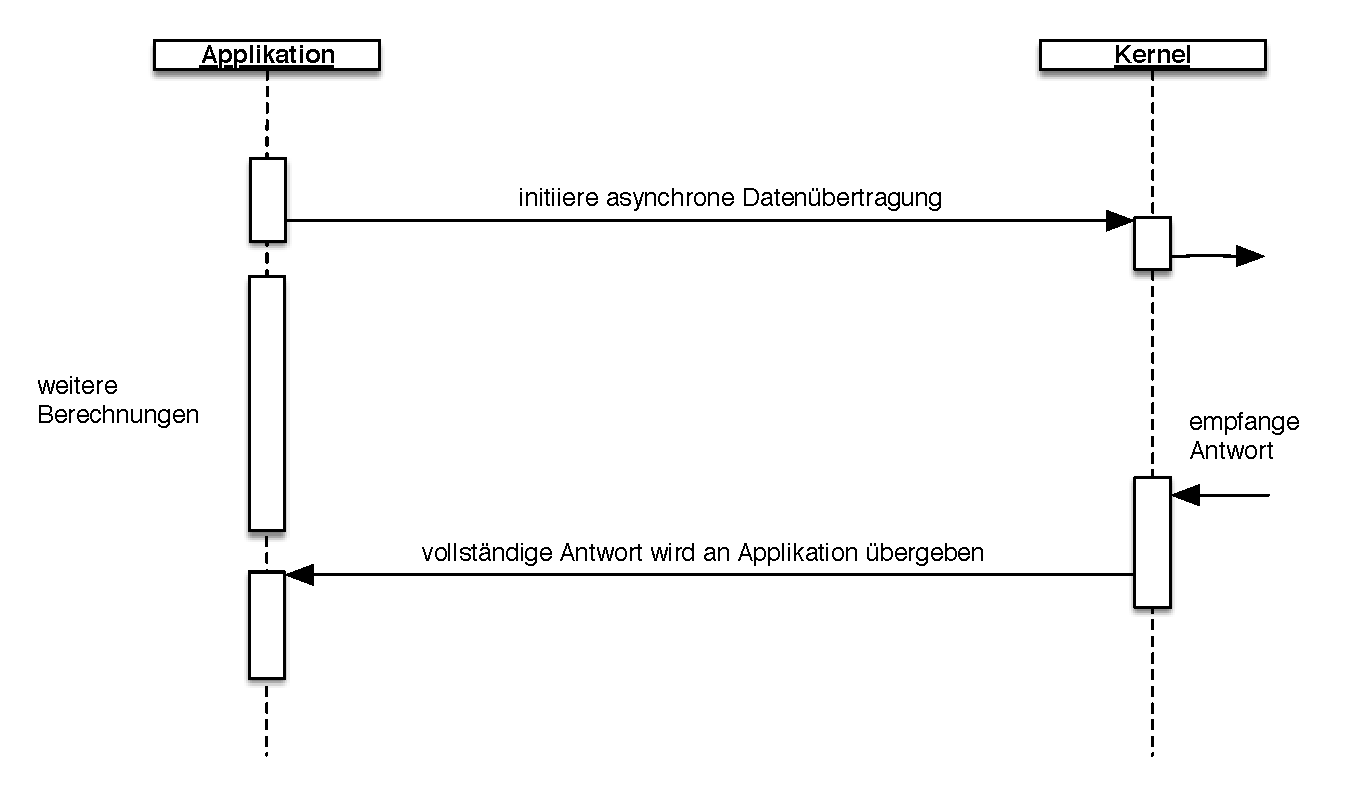
\includegraphics[width=1.0\textwidth]{4-Hauptteil/async-io/async-io.eps}
 \caption{Ablauf einer asynchronen und nicht blockierenden Datenübertragung}
 \label{fig:async-io}
\end{figure}

Die Anwendung kann nach der Initiierung der Datenübertragung sofort mit weiteren Berechnungen fortfahren. Das Betriebssystem informiert die Anwendung über die erfolgreiche Übertragung und übergibt die vollständige Antwort an die Anwendung. Durch diesen Mechanismus ist es möglich mit einem Thread mehrere Datenübertragungen asynchron abzuarbeiten, da diese den Thread nicht, wie traditionellerweise blockieren~\cite{jones_boost_2006}.

\pagebreak

Eine Webapplikation ist meist stark an Datenübertragung gebunden. Sei es die eigentliche HTTP Schnittstelle, der Zugriff auf die Datenbank oder die Kommunikation mit anderen Services. Eine Anfrage hat meist zur Folge, dass auf eine Datenbank zugegriffen wird. Die Ergebnisse der Datenbankanfrage werden aufbereitet und an den Client zurückgegeben. Der eigentliche Aufwand für die CPU ist relativ gesehen sehr gering.\\
Eine traditionelle Multi-threaded Webapplikation weist jeder eingehenden Anfrage einen dediziert Thread zu. Mit synchroner und blockierender Datenübertragung ist dieser Thread so lange blockiert bis die Antwort auf die Anfrage beim Client eingegangen ist. Ein Client mit einer langsamen Netzwerkanbindung blockiert deshalb einen Thread länger, wie ein Client mit einer schnellen Netzwerkanbindung.\\
Um eine Multi-threaded Webapplikation skalieren zu können, setzt man Thread pools ein, die eine vielzahl von Threads vorhalten --- meist weit aus mehr als der Prozessor Kerne hat. Jedoch ist die Koordination der Threads aufwendig und hat häufiges \textit{context switching} zur Folge.\\
Mit dem Modell der asynchronen und nicht blockierenden Datenübertragungen lassen sich Ressourcen effizienter nutzen. Zudem erhält man eine bessere vertikale Skalierung, als beispielsweise beim beschriebenen \enquote{One thread per request} Modell~\cite[S.~171]{butcher_seven_2014}~\cite[S.~76]{erb_concurrent_2012}.

\pagebreak

\subsection{Ereignisbasierte Concurrency}
Viele Anwendungen nutzen das Konzept der Events, um den Ablauf der Ausführung zu steuern. Man spricht auch von ereignisorientierter Software.\\ 
Ein Event ist ein Ereignis respektive ein Signal über eine Zustandsänderung. Im Gegensatz zu einer Nachricht hat ein Event keinen expliziten Empfänger, also keine Zieladresse. Komponenten können sogenannte Event handler an einem System registrieren. Diese werden dann über Zustandsänderungen informiert bzw. aufgerufen. Solange es zu keiner Zustandsänderung kommt, wird auch kein Event handler aufgefordert, ein Event zu verarbeiten. Die Komponente bleibt somit inaktiv~\cite[S.~91]{erb_concurrent_2012}.

\subsubsection{Reactor Pattern}
Ereignisorientierte Anwendungen müssen in der Regel viele Events von vielen verschiedenen Quellen koordinieren und abarbeiten. Beispielsweise ist jede Anfrage an eine Webanwendung ein Event und jeder Client folglich eine Quelle. Die Anfragen bzw. die Events können auch parallel bei der Anwendung eintreffen.\\
Um die Events abzuarbeiten, wird oft auf das Reactor Pattern zurückgegriffen (\autoref{fig:event-loop}). Events aus verschiedensten Quellen werden serialisiert und Event für Event abgearbeitet bzw. an die entsprechenden Event handler übergeben. Die Ausführung der Event handler erfolgt synchron. Die Reactor Komponente arbeitet in einer Endlosschleife, genannt Event loop~\cite[S.~260~-~S.~261]{buschmann_pattern_2011}.

\begin{figure}[H]
 \centering
 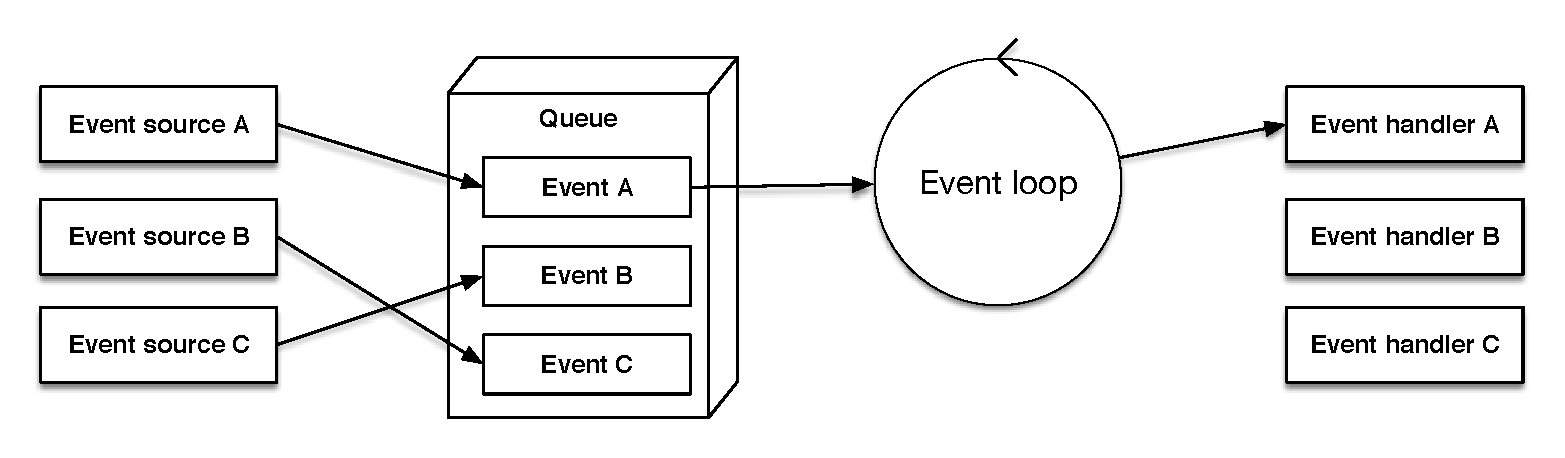
\includegraphics[width=1.0\textwidth]{4-Hauptteil/event-loop/event-loop.eps}
 \caption{Graphische Darstellung der Funktionsweise des Reactor Patterns}
 \label{fig:event-loop}
\end{figure}

Die Event loop wird typischerweise von genau einem Thread ausgeführt. Um dennoch nebenläufig mehrere Anfragen verarbeiten zu können, nutzt man Asynchronous I/O (siehe \autoref{subsec:async-io}). So ist es möglich nebenläufig, mit nur einem Thread, auf Events von vielen verschiedenen Quellen zu reagieren. Ein Event handler blockiert während der synchronen Ausführung, die Event loop und somit die Abarbeitung weiterer Events. Folglich ist das Reactor basierte Concurrency Modell nur für datenübertragungsintensive Applikationen, die von Asynchronous I/O profitieren, sinnvoll~\cite[S.~73]{kuhn_reactive_2015}~\cite[S.~92]{erb_concurrent_2012}.\\
Mit dem Reactor Pattern ist es möglich viele Anfrage nebenläufig, mit nur einem Thread, zu verarbeiten. Es entsteht kein Performance Overhead, wie bei traditionellen \enquote{One thread per request} Applikationen. Zudem wird die Komplexität der nebenläufigen Verarbeitung in der Reactor Komponente gekapselt und der Entwickler muss nicht mit den typischen Problemen der nebenläufigen Programmierung kämpfen. Außerdem können Event handler leicht wiederverwendet und kombiniert werden.\\
Es gibt zwei populäre Implementierungen dieses Concurrency Modells. Zum einen das JavaScript (V8) basierte Node.js\footnote{https://nodejs.org} und zum anderen das JVM basierte Vert.x\footnote{http://vertx.io}. Beide implementieren das Reactor Pattern unterscheiden sich jedoch in ihrer Anwendbarkeit für reaktive Anwendungen.\\
Vert.x bietet dem Entwickler die Möglichkeit über einen verteilten Event Bus eine Applikation message-driven zu implementieren. Zudem skaliert Vert.x auf einem Multi-core Prozessor besser, wie das Single-Threaded Node.js. Vert.x startet in der Standardeinstellung mehrere Event loops --- so viele, wie der Prozessor Cores hat --- und nennt dieses Konzept Multi-Reactor Pattern. Durch diese beiden Mechanismen, dem verteilten Event Bus, sowie dem Multi-Reactor Pattern, ist es möglich vertikal und horizontal zu skalieren. Unter dieses Gesichtpunkten eignet sich Vert.x als Basis Framework zur Entwicklung von reaktiven Anwendungen~\cite[S.~74]{kuhn_reactive_2015} \cite[S.~93~\&~S.~94]{erb_concurrent_2012}.

\pagebreak

\subsection{Actor-basierte Concurrency}
Im folgenden Abschnitt wird ein weiteres Concurrency Modell als Basis für reaktive Software vorgestellt.\\
Actor-basierte Concurrency oder kurz das \enquote{Actor Modell} stammt ursprünglich von Dr. Carl Hewitt et al aus dem Jahr 1973~\cite{hewitt_universal_1973}. Die grundlegende Idee des Actor Modells, ist die Abstraktion der Concurrency durch asynchronen Nachrichtenausstausch zwischen Komponenten. Eine Komponente in einer Actor-basierten Anwendung wird Actor genannt. Alan Kay, bekannt für seine Pionierarbeit zu objektorientierter Programmierung und außerdem einer der Entwickler der einflussreichen Sprache Smalltalk, sagt in einem Interview folgendes über das Actor Modell~\cite{binstock_interview_2012}:

\begin{quotation}
[...] the Actor model retained more of what I thought were the good features of the object idea [...]
\end{quotation}

Kay bezog sich dabei auf die geläufige Interpretation objektorientierter Programmierung, wie sie beispielsweise in C++ oder Java umgesetzt wurde. Der Kerngedanke der objektorientierten Programmierung müsste vielmehr die Kommunikation zwischen den Komponenten sein und sollte den Fokus nicht auf die Attribute oder das innere Verhalten der Objekte legen~\cite[S.~10]{vernon_reactive_2016}.\\
Das Actor Modell setzt im Grunde an diesem Gedanken an und lässt Komponenten über Nachrichten kommunizieren. 

\begin{figure}[H]
 \centering
 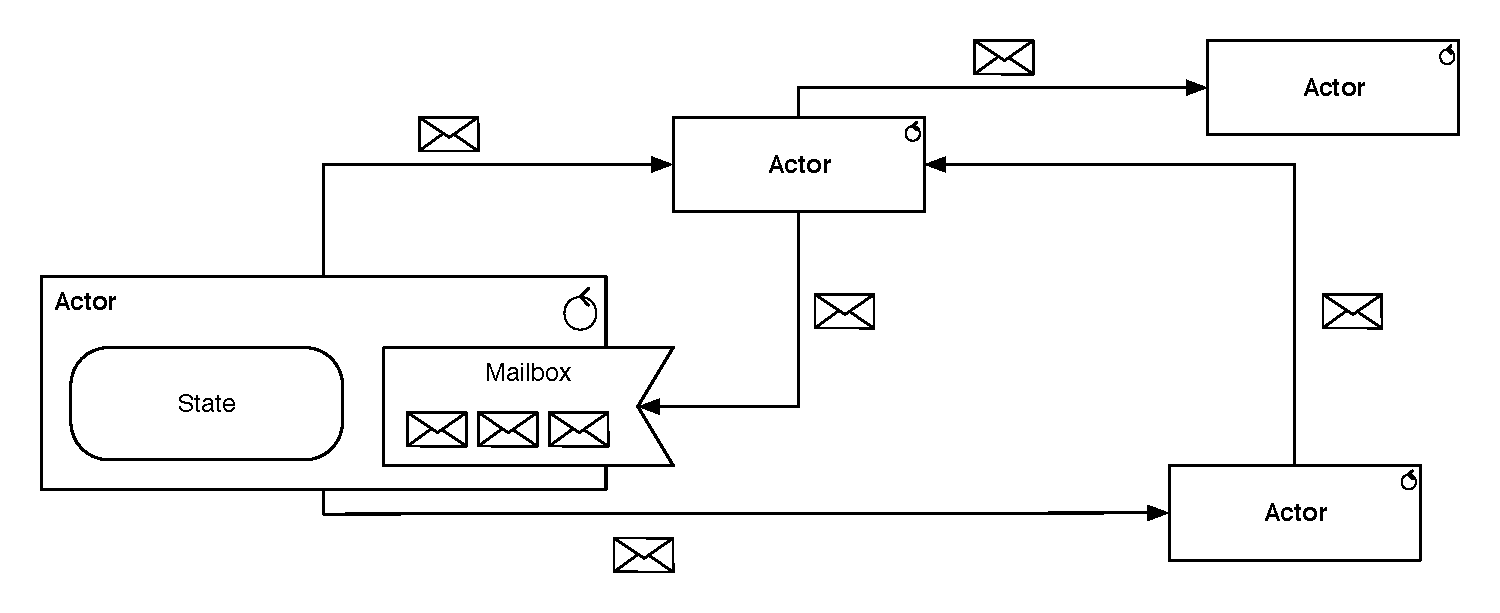
\includegraphics[width=1.0\textwidth]{4-Hauptteil/actor-model/actor-model.eps}
 \caption{Graphisches Beispiel einer Actor-basierten Anwendung.}
 \label{fig:actor-model}
\end{figure}

Ein Actor ist die kleinste Einheit in einer Actor-basierten Anwendung im Sinne des \enquote{Single Responsibility Principle} (siehe ???), wie das graphische Beispiel eines Bestellvorgangs (\ref{fig:actor-model}) zeigen soll. Jeder Actor besitzt eine sogenannte Mailbox, als Zwischenspeicher für eingehende Nachrichten, und einen Namen bzw. eine Adresse. Um nun einem Actor eine Nachricht zu schicken, wird die Adresse des Actors benötigt. Die Übertragung eine Mailbox ist von unbestimmter Dauer. Zudem wird keine Reihenfolge der eingetroffenen Nachrichten garantiert~\cite[S.~84]{erb_concurrent_2012} \cite[S.~83]{kuhn_reactive_2015}.\\
Ein Actor arbeitet jede Nachricht aus der Mailbox sequenziell ab. Deshalb muss während der Verarbeitung nicht auf Probleme bzgl. Nebenläufigkeit geachtet werden.\\
Ein Actor kann auf drei verschiedene Weisen auf eine Nachricht reagieren \cite[S.~84]{erb_concurrent_2012}:

\begin{enumerate}
\item Verschickt eine begrenzte Anzahl von Nachrichten an andere Akteure.
\item Erzeugt eine begrenzte Anzahl weiterer Akteure.
\item Ändert den eigenen internen Zustand in Folge der empfangenen Nachricht.
\end{enumerate}

Der Zustand eines Actors ist isoliert und kann nur von dem Actor selbst verändert werden. Zustandsänderungen und daraus resultierende Verhaltensänderungen wirken sich erst auf nachfolgende Nachrichten aus.\\
Actor-basierte Anwendung setzen somit auf \textit{mutable state} --- jedoch wird dieser nicht geteilt. Ein Actor kapselt seinen Zustand und interagiert nur über Nachrichten mit anderen Akteure.

Das Actor Modell wurde poplär durch die Programmiersprache Erlang\footnote{https://www.erlang.org/} und das Framework Akka\footnote{http://akka.io}.

\pagebreak

\section{Reaktive Programmierung}
Reaktive Programmierung, im weiteren Sinne, ist in der Entwicklung von Benutzeroberflächen üblich und verbreitet. Eine Software mit Benutzernutzeroberfläche muss stetig auf Eingaben durch den Benutzer reagieren. Dazu gehören neben Tastatureingaben und Mausklicks auch Cursorbewegungen. Dieser stetige Strom von neuen Informationen und Ereignissen muss verarbeitet werden, ohne dabei die Benutzeroberfläche zu blockieren. Nichts ist ärgerlicher, als eine Software, die nach einem Klick auf einen Button nicht reagiert bis der Vorgang abgeschlossen ist. Ebenso verhält sich es mit Serveranwendungen, die auf eine Vielzahl von gleichzeitigen Anfragen reagieren müssen.\\
Zu Beginn der Arbeit wurde bereits die Definition reaktiver Systeme von Harel und Pnueli genannt. Allgemeiner betrachtet bedeutet das englische Wort \textit{reactive} laut dem Merriam-Webster Wörterbuch \enquote{readily responsive to a stimulus}. Demnach ist etwas \textit{reactive}, wenn es bereitwillig auf einen Reiz reagiert. Im Bezug auf Software sind Reize beispielsweise Cursorbewegungen, Mausklicks oder Anfragen. Konkreter formuliert sind diese Reize Ereignisse, die von einer Komponente verarbeitet werden. Folgich ist ein Ereignis (engl. event) ein Signal über eine Zustandsänderung. Eine Komponente sendet ein Ereignis an seine Empfänger. Die reaktive Programmierung beschäftigt sich mit der nebenläufigen und asynchronen Verarbeitung dieser Ereignisse, um die \textit{responsiveness} der Anwendung sicherzustellen~\cite{rappl_introduction_2016}~\cite[S.~4]{carkci_dataflow_2014}~\cite[S.~5]{blackheath_functional_2015}.

\section{Observer-Pattern}
Ein Ereignis (engl. event) ist ein Signal bzw. ein Fakt über eine Zustandsänderung. Eine Komponente emittiert bzw. veröffentlicht ein Ereignis an seine Empfänger bzw. Beobachter. Hierfür nutzt man traditionellerweise das Verhaltensmuster \textit{observer}. Ein Beobachter (engl. observer) hat die Möglichkeit sich für Zustandsänderungen an- und abzumelden.\\
Folgendes Scala Codebeispiel zeigt das Observer-Pattern durch das Trait \textit{EventEmitter} (\ref{lst:lst5}). Beobachter, im Codebeispiel \textit{Observer} genannt, können sich über die Methoden \textit{subscribe} und \textit{unsubscribe} beim \textit{EventEmitter} an- und abmelden. Kommt es zu einer Zustandsänderung kann der \textit{EventEmitter} alle \textit{Observer} durch den Aufruf von \textit{emit} über das Ereignis informieren. Der \textit{EventEmitter} weiß nur, dass die \textit{Observer} die Methode \textit{handle} implementieren, die durch \textit{emit} aufgerufen wird.

\begin{lstlisting}[caption={Codebeispiel für das Observer-Pattern.},label={lst:lst5}]
trait EventEmitter {
  private var observers: Set[Observer] = Set()

  def subscribe(observer: Observer): Unit = observers += observer
  def unsubscribe(observer: Observer): Unit = observers -= observer
  def emit(): Unit = observers.foreach(_.handle(this))
}

trait Observer {
  def handle(emitter: EventEmitter): Unit
}
\end{lstlisting}

\pagebreak

\begin{lstlisting}[caption={Codebeispiel für das Observer-Pattern.},label={lst:lst6}]
class IncrementButton extends EventEmitter {
  private var counter = 0

  def getCount = counter
  def clicked(): Unit = {
    counter += 1
    emit()
  }
}

class IncrementLogger(button: IncrementButton) extends Observer {
  button.subscribe(this)

  def handle(emitter: EventEmitter): Unit = println(s"new value \${button.count}")
}

val button = new IncrementButton()
val logger = new IncrementLogger(button)

button.clicked() // prints: new value 1
button.clicked() // prints: new value 2
button.clicked() // prints: new value 3
button.clicked() // prints: new value 4
\end{lstlisting}

\subsection{Messages \& Events}
Ein reaktives System ist \textit{message-driven}, folglich nutzt es asynchrone Nachrichtenübermittlung (engl. message passing) zur Kommunikation zwischen den Komponenten. Eine Nachricht (engl. message) wird von seinem Sender an einen Empfänger geschickt. Eine Nachricht enthält somit eine Zieladresse und Daten. Die Komponenten müssen folglich adressierbar sein und auf reagieren nur auf für sie bestimmte Nachrichten. Trifft keine Nachricht für eine Komponente ein, bleibt diese inaktiv.

% Enterprise Integration Patterns: Message, Message Channel, Event Message, Event-Driven Consumer

% Ein Ereignis (engl. event) ist ein Signal bzw. ein Fakt über eine Zustandsänderung.

\subsection{Observables}
%TODO Reactive extensions & Observable 
%TODO Deprecating the Observer Pattern
%TODO Erik Meijer Talk about What is reactive?
%TODO Lesli Lamport We should use mathematics!
%TODO Rx are libraries for asynchronous and therefore reactive programming.

\pagebreak

\section{Reactive Design Patterns}
\subsection{Actor Model}
\subsection{Reactive Streams}
\subsection{Circuit Breaker}

\section{Implementierung}
\subsection{Akka (Scala)}
\subsection{NodeJS (JavaScript)}

\section{Ergebnisse}
\subsection{Nutzen der Patterns}
\subsection{Einfachheit der Implementierung}
\subsection{Unterstützung durch Frameworks}


% Ergebnisse
% !TEX root = ../Masterdatei.tex
\chapter{Schluss}

\section{Reaktive Systeme}
\subsection{Microservices}
\subsection{12-Factor Applications}

\section{Zusammenfassung}


% BibTex
\nocite{*}
\bibliographystyle{alphadin}
\bibliography{0-Template/Bibliothek.bib}{}

% Verzeichnisse
\listoffigures
\listoftables
\printglossary[type=main, title=Glossar,toctitle=Glossar]
\printglossary[type=acronym, title=Akronyme,toctitle=Akronyme]

\end{document}
